\begin{frame}
\frametitle{EuGENia Case Study}

\begin{itemize}
\item EuGENia creates a GMF editor from an Ecore metamodel
\item It is written in EOL
\item It has an EUnit test suite
\end{itemize}

\begin{figure}
	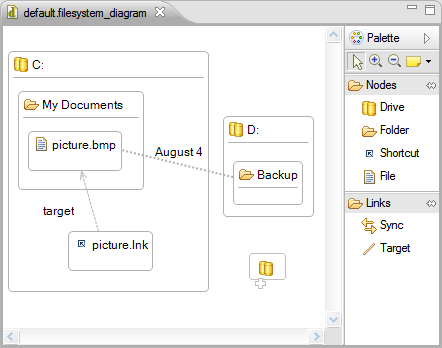
\includegraphics[width=2in]{figures/gmfeditor.png}
\caption{A sample gmf editor generated by EuGENia}
\end{figure}

\end{frame}

\begin{frame}
\frametitle{EuGENia Case Study - Statement Coverage}
\begin{itemize}
\item 49\% Statement Coverage
\end{itemize}

\begin{figure}
	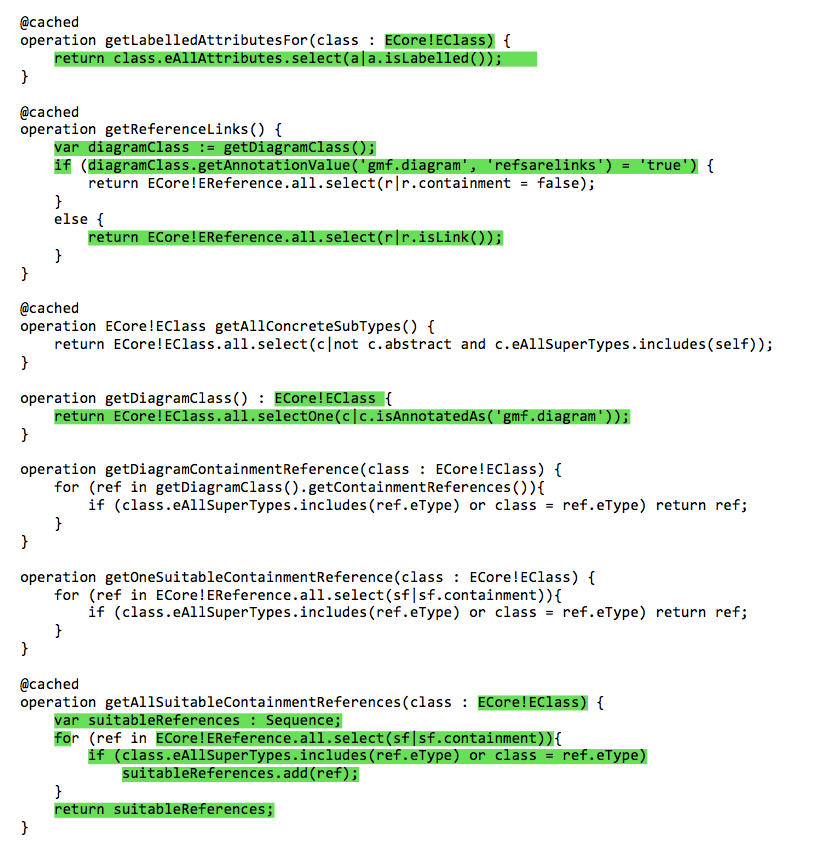
\includegraphics[scale=0.3]{./presentation/images/eugenia_statement_coverage.png}
\end{figure}
\end{frame}

\begin{frame}
\frametitle{EuGENia Case Study - Branch Coverage}
\begin{itemize}
\item 61\% Branch Coverage
\end{itemize}

\begin{figure}
	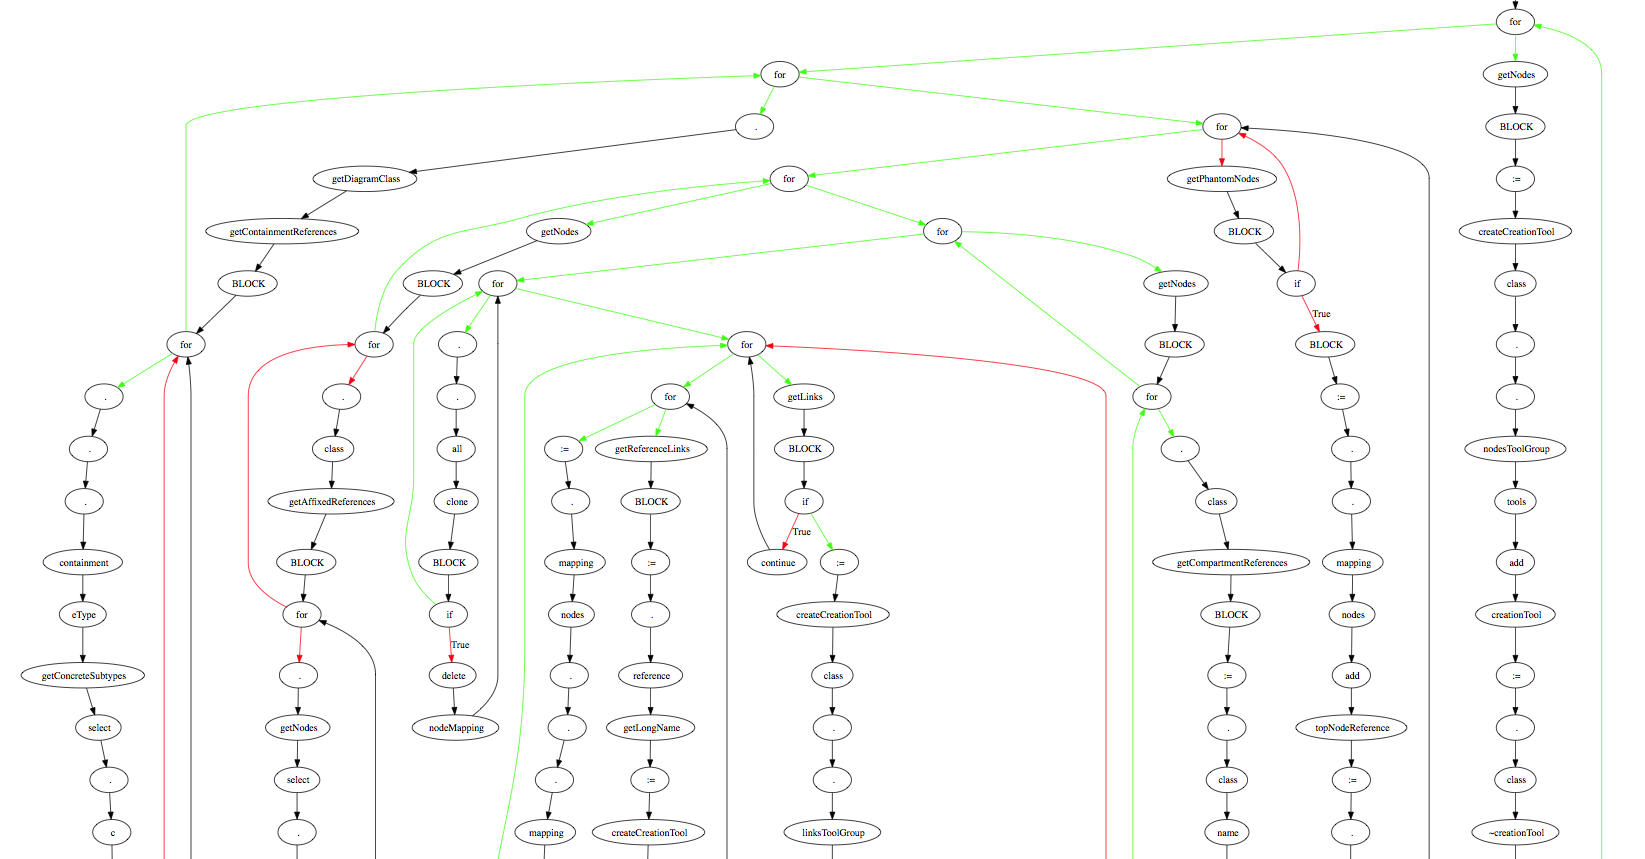
\includegraphics[scale=0.3]{./presentation/images/eugenia_branch_coverage.png}
\end{figure}
\end{frame}

\begin{frame}
\frametitle{EuGENia Case Study - Performance}
\begin{table}
\centering
    \begin{tabular}{|p{0.75in} | p{0.5in} |p{0.5in} |p{0.5in} |p{0.5in} |p{0.65in} |} \hline
    Coverage Type & Time 1 (s) & Time 2 (s) & Time 3 (s) & Average Time (s) & Standard Deviation (s) \\\hline
    None          & 56.9             & 52.4             & 53.6             & 54.3                   & 2.3                          \\\hline
    Statement     & 62.9             & 63.2             & 62.3             & 62.8                   & 0.5                          \\\hline
    Branch        & 68.4             & 65.9             & 65.7             & 66.7                   & 1.5                          \\\hline
    \end{tabular}
    \caption{Run times of the EuGENia test suite}
    \label{tab:runTimes}
\end{table}
\begin{itemize}
\item Statement Coverage +15\%
\item Branch Coverage +23\%
\end{itemize}
\end{frame}

